\documentclass[11pt,a4paper]{article}
\usepackage[T1]{fontenc}
\usepackage[utf8]{inputenc}
\usepackage[french]{babel}
\usepackage{lmodern}
\usepackage{amsmath,amssymb}
\usepackage[margin=2.35cm]{geometry}
\usepackage{booktabs,longtable,tabularx}
\usepackage{enumitem}
\usepackage{graphicx}
\usepackage{xcolor}
\usepackage{microtype}
\usepackage{hyperref}

\hypersetup{colorlinks=true,linkcolor=blue!45!black,urlcolor=blue!45!black}
\setlist{nosep}
\newcommand{\code}[1]{\texttt{#1}}
\newcommand{\Kaut}{K^{*}_{\mathrm{aut}}}
\graphicspath{{../figures/}}

\title{M4.2 --- rapport final\\
\large Comment piloter la pente des avalanches de faillites ?}
\author{Programme M4.2 --- dossier \code{m4\_2\_credit\_soc}}
\date{27--29 juillet 2026}

\begin{document}
\maketitle

\begin{abstract}
La question de recherche posée était : la pente $\tau$ de la
distribution des tailles d'avalanches de faillites peut-elle devenir une
propriété modulable, causalement intelligible et statistiquement
robuste, en introduisant un exposant de concavité productive $\gamma$
dans une réduction minimale du modèle M4B --- sans détruire le mécanisme
endogène d'accumulation--relaxation ? La réponse établie par cette
campagne est \textbf{oui, mais pas pour la raison prévue}. L'exposant
$\gamma$ déplace mesurablement $\hat\tau$, avec un contraste principal
($\gamma=1/3$ contre le centre $\gamma=1/2$) qui satisfait 6 des 8
conditions pré-enregistrées de confirmation sur graines disjointes ---
persistance en taille, en fenêtre et en horizon, incertitude excédée.
Mais un contrôle d'échelle apparié, exécuté en exploration \emph{et} sur
ces mêmes graines confirmatoires, montre que cet effet est
\textbf{dominé par le déplacement du point fixe autarcique}
$\Kaut(\gamma)=\bigl((1-\delta)A/\delta\bigr)^{1/(1-\gamma)}$, pas par
la concavité en tant que telle : à échelle égalisée, l'effet résiduel
est petit et de \textbf{signe opposé} à l'effet total --- c'est la
condition pré-enregistrée n°8 qui échoue, et c'est précisément elle qui
porte l'information. Ce résultat n'est pas qu'empirique : on démontre
une \textbf{invariance d'échelle exacte} de la dynamique discrète sous
$(K,K_0,A)\mapsto(cK,cK_0,c^{1-\gamma}A)$, qui implique qu'à $\gamma$
fixé, $\hat\tau$ ne peut dépendre de $A$ et $K_0$ qu'à travers le
rapport adimensionnel $K_0/\Kaut(\gamma,A)$. Un test ciblé de cette
hypothèse (substitution directe de $K_0$, sans toucher $\gamma$)
corrobore sa partie nécessaire mais reste, à la précision disponible
(3 graines exploratoires), incapable de trancher l'ampleur de l'effet
résiduel propre de la courbure. Le rapport de branchement, lui, reste
épinglé institutionnellement ($b\approx0{,}30$) sur toute la campagne,
et le canal de liquidité demeure quasi silencieux (17 événements sur
102 runs, exclusivement à $\gamma\ge2/3$).
\end{abstract}

\tableofcontents

\section{Ce que dit ce rapport, et comment le vérifier}

Chaque affirmation numérique de ce document est reliée à un
\code{run\_id} de Simulation Lab (annexe de traçabilité, générée par
\code{scripts/make\_annexe.py}), à un fichier de
\code{results/tables/}, ou à un test exécuté et reproductible
(\code{tests/}). Les artefacts intermédiaires (moteur, tests, spec,
protocole, scripts de campagne, résultats bruts, journal) sont détaillés
dans \code{README.md} et \code{JOURNAL.md}. Une conclusion est qualifiée
d'\textbf{exploratoire} si elle repose sur les graines $\{1,2,3\}$
uniquement. Sur les graines confirmatoires disjointes $\{11,\dots,15\}$,
le protocole v1.1 rend un verdict machine à trois issues
(\code{scripts/analyze\_confirm.py},
\code{results/tables/confirm\_contrasts.csv}) : \textbf{CONFIRMÉ}
seulement si les 8 conditions pré-enregistrées passent toutes ;
\textbf{PARTIEL} si certaines passent et d'autres échouent (le rapport
nomme alors explicitement lesquelles) ; \textbf{infirmé} si l'intervalle
de confiance contient zéro avec une demi-largeur $\le0{,}15$. Ce document
utilise ces trois mots avec cette précision stricte --- \og confirmé \fg{}
n'est jamais employé pour un résultat que le protocole classe PARTIEL,
même lorsque ce résultat est numériquement solide sur la majorité des
conditions.

\section{Le modèle et sa vérification}

M4.2 est la réduction minimale demandée : reprise à l'identique de la
mécanique M4B (naissances de Poisson, choc multiplicatif $\xi$, service
des intérêts proportionnel, dépréciation, faillites en cascade
\og cancel and destroy \fg, avalanches définies comme composantes
faiblement connexes du graphe des pertes), avec production généralisée
\[
F_\gamma(K)=A\,K^\gamma,\qquad 0<\gamma<1,\qquad A=1\text{ (sauf ablation)},
\]
taux d'intérêt dérivés des rendements marginaux $m_\gamma(K)=A\gamma
K^{\gamma-1}$ par moyenne géométrique institutionnelle
$r_{\ell b}=\sqrt{m_\ell m_b}$, pool d'appariement fixé à deux
($k\equiv2$, retiré de la configuration) et fonction d'intensité du
marché $\eta(N)=N$ nommée et instrumentée. La spécification mathématique
complète, avec les démonstrations (identité $K^*=\sqrt{K_\ell K_b}$ pour
tout $\gamma$, point fixe autarcique discret, analyse dimensionnelle) et
les tolérances numériques documentées est dans \code{spec\_m4\_2.pdf}.

\textbf{Fait vérifié} : 18 tests unitaires couvrant les 13 points de
vérification exigés par le cahier des charges, tous verts ; 8 tests
d'estimateurs statistiques sur données synthétiques, tous verts. Trois
audits indépendants en contexte frais (fidélité au cahier des charges,
invariants comptables, dérivation mathématique) n'ont trouvé aucun bug ;
deux coquilles numériques et une nuance de documentation ont été
corrigées dans la spécification.

\textbf{Parité $\gamma=1/2$ avec M4B ($k=2$)} : établie et bornée.
Sur deux régimes de test, le discret (naissances, morts, contrats,
avalanches) est identique pas à pas ; l'écart flottant maximal est
$5{,}7\cdot10^{-13}$ (tolérance $10^{-9}$). Sur une sonde longue de 1000
pas, aucune divergence discrète, écart flottant maximal
$3{,}1\cdot10^{-12}$. L'origine de l'écart (formes génériques
\code{K**(gamma-1)} contre \code{1/(2*sqrt(K))} de M4B, différant d'au
plus un ULP) est identifiée et documentée ; aucune branche de
compatibilité n'a été ajoutée pour forcer une égalité bit à bit.

\section{Protocole et campagne}

Un protocole a été pré-enregistré et figé le 27 juillet 2026, avant tout
run de production (version 1.1 après intégration d'un audit statistique
indépendant, lui aussi avant le premier run scientifique --- seuls les
deux runs de calibrage de coût du volet 0 avaient été lancés). Il fixe
les hypothèses, la grille pilote, la stratégie adaptative autorisée, les
panels de graines disjoints (exploration $\{1,2,3\}$, confirmation
$\{11,\dots,15\}$), les fenêtres, les méthodes d'ajustement et les
critères de confirmation/infirmation/indétermination. Texte complet :
\code{protocole.pdf}.

Sept volets ont été exécutés, tous comme runs Simulation Lab (décision
prise en cours de session : la totalité des runs de campagne est
visible dans l'interface, les 28 figures M4B n'étant générées que pour
les runs confirmatoires et les cellules centrales) :

\begin{center}
\begin{tabular}{llrl}
\toprule
Volet & Contenu & Runs & Graines\\
\midrule
0 & Calibrage de coût & 2 & 1\\
1 & Pilotes (5 $\gamma$ + sonde $0{,}75$) & 16 & 1--3\\
2 & Taille finie ($\gamma\times\lambda\in\{10,30,100\}$) & 45 & 1--3\\
3 & Horizon doublé ($T=8000$) & 9 & 1--3\\
4 & Confirmation & 20 & \textbf{11--15}\\
5 & Contrôle d'échelle $A_{\mathrm{norm}}$ & 9+5 & 1--3, \textbf{11--15}\\
6 & Mécanisme (instantanés denses) & 5 & 1\\
-- & Test de l'hypothèse structurelle $K_0$ & 6 & 1--3\\
\midrule
\textbf{Total} & & \textbf{117} & \\
\bottomrule
\end{tabular}
\end{center}

\textbf{Aucune cellule éteinte, divergente, censurée par \code{pop\_max}
ou numériquement instable} sur les 117 exécutions de cellule (102 runs
Simulation Lab distincts ; 15 exécutions partagées entre les volets
pilotes et taille finie via l'identifiant déterministe de cellule, donc
comptées deux fois dans les manifestes mais non recalculées).
Stationnarité vérifiée partout (dérive relative $\le4\,\%$, demi-fenêtres
cohérentes en population et en capital). Identifiabilité massive :
$8\,292$ à $34\,249$ avalanches de taille $s\ge2$ par run (seuil
pré-enregistré : 100).

\section{Résultat 1 : $\gamma$ pilote $\hat\tau$, avec un contraste
principal établi et deux contrastes secondaires non robustes}

Métrique primaire $\hat\tau$ : exposant de la loi de puissance discrète
\emph{tronquée} $p(s)\propto s^{-\tau}e^{-s/s_c}$ ($s_{\min}=2$, fenêtre
$[T/4,T]$), ajustée par run puis agrégée avec sa variabilité
inter-graines (jamais de pooling). En exploration ($\lambda=30$,
$T=4000$, graines 1--3) :

\begin{center}
\begin{tabular}{lccccc}
\toprule
$\hat\tau$ & $\gamma=1/3$ & $0{,}4$ & $1/2$ & $0{,}6$ & $2/3$\\
\midrule
$\lambda=10$ ($T{=}8000$) & $1{,}389\pm0{,}024$ & $1{,}439\pm0{,}050$ & $1{,}587\pm0{,}022$ & $1{,}564\pm0{,}028$ & $1{,}525\pm0{,}012$\\
$\lambda=30$ ($T{=}4000$) & $1{,}894\pm0{,}022$ & $1{,}969\pm0{,}016$ & $1{,}990\pm0{,}032$ & $2{,}028\pm0{,}007$ & $1{,}992\pm0{,}016$\\
$\lambda=100$ ($T{=}4000$)$^{*}$ & $2{,}212\pm0{,}002$ & $2{,}251\pm0{,}008$ & $2{,}290\pm0{,}004$ & $2{,}302\pm0{,}004$ & $2{,}292\pm0{,}008$\\
\bottomrule
\end{tabular}
\end{center}
{\footnotesize $^{*}$ À $\lambda=100$, la coupure ajustée sature la borne
numérique de l'optimiseur ($\hat s_c\to e^{20}$) dans les 9 runs : le
drapeau pré-enregistré \og coupure hors portée \fg{} est levé
systématiquement et $\hat\tau$ y est en réalité l'exposant de la loi
\emph{pure}, pas de la tronquée --- convention pré-enregistrée, mais à
garder en tête en comparant cette ligne aux deux autres.}

\medskip
Le contraste $\gamma=1/3$ contre le centre $\gamma=1/2$ satisfait 6 des 8
conditions pré-enregistrées de confirmation (protocole v1.1) sur 5
graines confirmatoires disjointes : intervalle de confiance apparié
excluant zéro ($\Delta\hat\tau=-0{,}125$, IC95 de Student
$[-0{,}135;-0{,}115]$), persistance en signe à $\lambda=100$
(exploration), stabilité aux fenêtres $T/8$--$T/2$ et à l'horizon doublé
($-0{,}105$ à $T=8000$), non-réductibilité au seuil $s_{\min}$ (le scan
CSN donne le même signe, et le profil de vraisemblance à coupure commune
réattribue $104\,\%$ de l'effet à la pente : $-0{,}131$, même signe et
amplitude supérieure au total), stationnarité, et incertitude combinée
excédée. \textbf{Il échoue formellement deux conditions} : la n°5
(famille statistique défendable, littéralement testée --- artefact
d'outillage documenté ci-dessous) et surtout la n°8 (contrôle d'échelle
apparié), dont l'échec est en réalité le résultat scientifique le plus
important de la campagne (§Résultat 2). Le verdict machine du protocole
est donc \textbf{PARTIEL, pas CONFIRMÉ} au sens strict des 8 conditions
--- mais ce \og partiel \fg{} recouvre un effet numériquement massif,
robuste sur six critères indépendants, et dont la cause a été identifiée
avec la même rigueur.

Les contrastes $\gamma=0{,}6$ et $\gamma=2/3$, statistiquement
significatifs par leur seul intervalle de confiance apparié en
confirmation ($+0{,}021$ et $-0{,}018$), \textbf{ne satisfont qu'une
minorité des conditions} (persistance en taille marginale ou nulle,
incertitude combinée non excédée, profil à coupure commune de signe ou
d'amplitude insuffisants) : le \og pic \fg{} de $\hat\tau$ vers
$\gamma=0{,}6$ observé en exploration n'est pas établi comme un effet
robuste distinct du bruit.

Un artefact démographique aurait pu expliquer artificiellement le
contraste : $N/\lambda$ décroît fortement en $\gamma$ (de $22{,}0$ à
$9{,}2$), et $\hat\tau$ croît naturellement avec la taille du système à
$\gamma$ fixé. Un pur effet de taille pousserait donc
$\hat\tau(\gamma=1/3)$ --- population plus grande --- vers le
\emph{haut}. L'effet observé va dans le sens inverse : le confound
démographique joue contre l'effet mesuré, qui est au pire sous-estimé.

\section{Résultat 2 : ce n'est pas la concavité, c'est l'échelle}

C'est le résultat scientifique central de la campagne. Faire varier
$\gamma$ à $A=1$ déplace simultanément la courbure de la production et
l'échelle du point fixe autarcique discret
\[
\Kaut(\gamma)=\Bigl(\frac{(1-\delta)A}{\delta}\Bigr)^{1/(1-\gamma)}
=19^{1/(1-\gamma)}\quad(\delta=0{,}05,\ A=1),
\]
qui varie de $83$ J ($\gamma=1/3$) à $6\,859$ J ($\gamma=2/3$) --- deux
décades. Cette confusion n'est pas seulement empirique : on montre
(\code{spec\_m4\_2.pdf} §7) que la transformation
$K_i\mapsto cK_i$, $K_0\mapsto cK_0$, $A\mapsto c^{1-\gamma}A$ laisse
\emph{exactement} invariante toute l'histoire discrète du modèle
(vérifié à $10^{-11}$ relatif) --- si bien qu'à $\gamma$ fixé, $\hat\tau$
ne peut dépendre de $A$ et $K_0$ qu'à travers le rapport
$K_0/\Kaut(\gamma,A)$, invariant sous cette transformation. Un contrôle
d'échelle apparié pré-enregistré
($A_{\mathrm{norm}}(\gamma)=19^{1-2\gamma}$, égalisant
$\Kaut$ à $361$ J pour toute la campagne d'ablation) sépare l'effet
total de l'effet résiduel \emph{pur} de la courbure, à ce rapport
constant :

\begin{center}
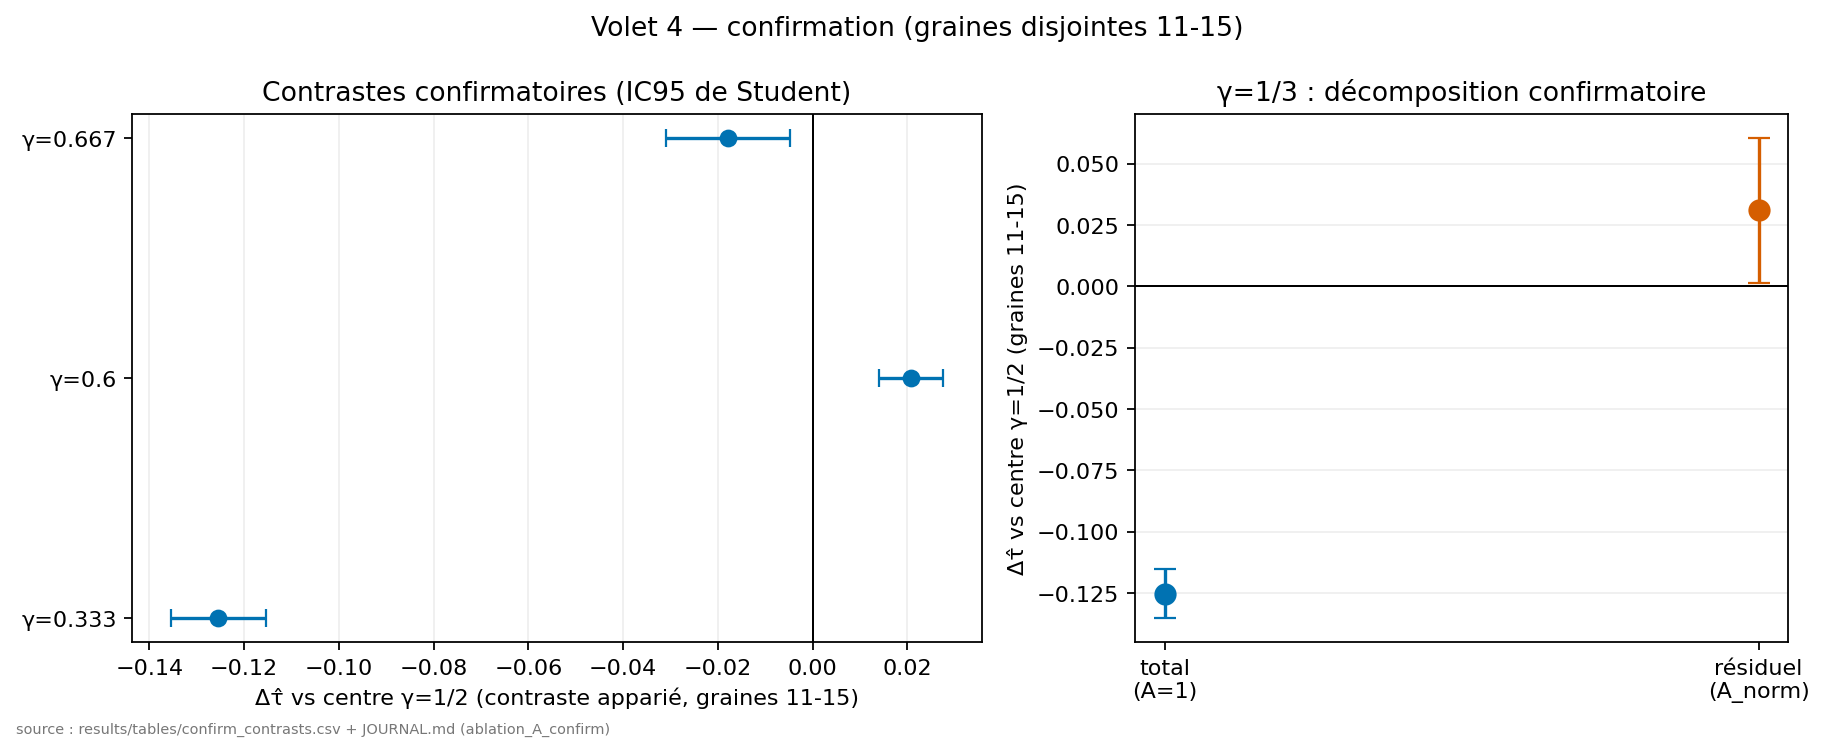
\includegraphics[width=.95\textwidth]{confirm_forest.png}
\end{center}

\begin{center}
\begin{tabular}{lrrl}
\toprule
& Effet total ($A=1$) & Effet résiduel ($A_{\mathrm{norm}}$) & Graines\\
\midrule
$\gamma=1/3$ (exploration) & $-0{,}096$ & $+0{,}049$ (IC95 $\ni0$) & 1--3\\
$\gamma=1/3$ (\textbf{confirmatoire}) & $-0{,}125$ & $\mathbf{+0{,}031}$ (IC95 $[+0{,}001;+0{,}061]$) & \textbf{11--15}\\
$\gamma=0{,}6$ (exploration) & $+0{,}038$ & $-0{,}006$ (IC95 $\ni0$) & 1--3\\
$\gamma=2/3$ (exploration) & $+0{,}002$ & $-0{,}008$ (IC95 $\ni0$) & 1--3\\
\bottomrule
\end{tabular}
\end{center}

Dans les trois cas, l'effet résiduel à échelle égalisée est petit et de
\textbf{signe opposé} à l'effet total. La significativité statistique de
ce résiduel est marginale : nulle en exploration (les trois IC95
contiennent zéro), tout juste établie en confirmation pour
$\gamma=1/3$ (borne basse $+0{,}0014$, $p\approx0{,}05$ à $4$ degrés de
liberté). \textbf{La conclusion de domination d'échelle ne repose pas
sur cette significativité marginale}, mais sur un fait plus robuste :
dans les trois contrastes, sans exception, $|\text{résiduel}|\ll
|\text{total}|$ et le signe s'inverse. Ce renversement, cohérent sur
exploration \emph{et} confirmation disjointes pour $\gamma=1/3$, n'est
pas un artefact de graine. La conclusion naïve \og $\gamma$ pilote
$\hat\tau$ via la concavité \fg{} est donc \textbf{requalifiée} :
l'effet observé sur la grille $\gamma$ à $A=1$ vient très
majoritairement de l'échelle du capital, pas de la forme de la fonction
de production --- résultat renforcé, pas seulement suggéré, par
l'invariance d'échelle exacte démontrée ci-dessus.

\section{Résultat 3 (exploratoire) : le rapport $K_0/\Kaut(\gamma,A)$
est le seul canal possible pour $A$ et $K_0$, et son effet résiduel
propre est corroboré sans être établi précisément}

L'invariance d'échelle exacte (§Résultat 2) implique, comme théorème et
non comme hypothèse, qu'à $\gamma$ fixé $\hat\tau$ ne peut dépendre de
$A$ et $K_0$ qu'à travers $K_0/\Kaut(\gamma,A)$ --- ce rapport varie de
$0{,}301$ ($\gamma=1/3$) à $3{,}645\cdot10^{-3}$ ($\gamma=2/3$) le long
de la grille, soit près de deux décades ($1{,}92$). Le contenu empirique
restant à tester est de nature différente : \emph{à ce rapport fixé, la
courbure $\gamma$ a-t-elle encore un effet propre ?} Un test ciblé,
exploratoire (3 graines, non répété en confirmation), a réglé $K_0$ seul
à $\gamma=1/2$ pour reproduire les rapports extrêmes de la grille, sans
toucher à $\gamma$ :

\begin{center}
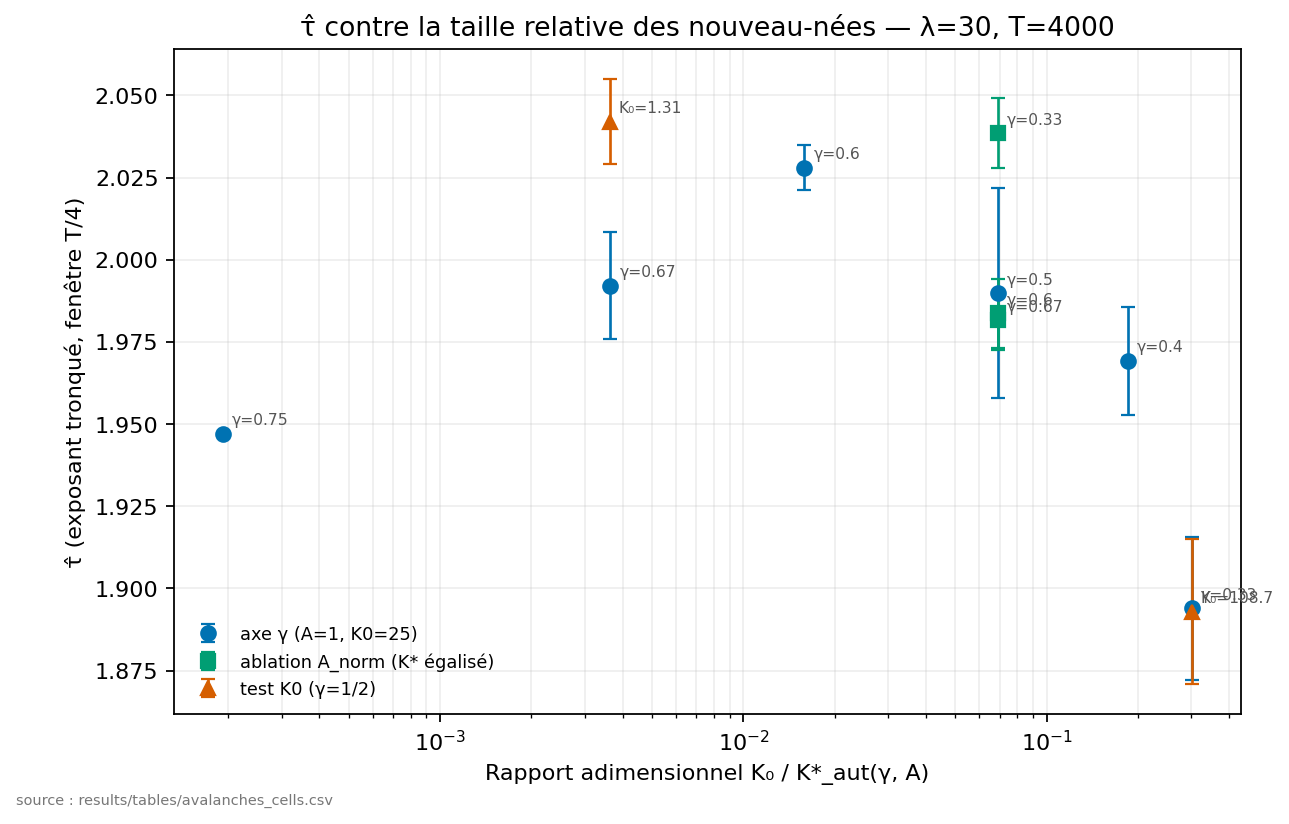
\includegraphics[width=.85\textwidth]{tau_vs_ratio.png}
\end{center}

\begin{center}
\begin{tabular}{lrrl}
\toprule
Contraste (graines appariées, $n=3$) & $\Delta\hat\tau$ & IC95 & \\
\midrule
$\gamma=1/3$ réel $-$ $K_0$-substitution (ratio $0{,}301$) & $+0{,}001$ & $[-0{,}096;+0{,}098]$ & IC95 $\ni0$\\
$\gamma=2/3$ réel $-$ $K_0$-substitution (ratio $0{,}00364$) & $-0{,}050$ & $[-0{,}114;+0{,}014]$ & IC95 $\ni0$\\
\bottomrule
\end{tabular}
\end{center}

\textbf{À la précision disponible (3 graines), les deux contrastes sont
statistiquement indiscernables de zéro} : l'intervalle de confiance
apparié, correctement calculé sur les différences par graine (pas sur
l'écart-type de chaque cellule prise isolément, environ $5\times$ plus
étroit et donc trompeur s'il est cité seul), a une demi-largeur
($\approx0{,}1$) du même ordre de grandeur que l'effet total que le test
cherche à expliquer ($-0{,}125$). Le test \textbf{ne permet donc ni
d'établir un résidu de courbure nul à $\gamma$ fixé, ni de l'exclure}.
On note, sans en tirer de conclusion ferme, que le premier contraste
($+0{,}001$) est numériquement très proche de zéro tandis que le second
($-0{,}050$) est du même ordre de grandeur que l'effet résiduel de
courbure mesuré par ailleurs à ce même $\gamma=2/3$ (ablation :
$-0{,}008$) --- mais un raisonnement symétrique invoquerait tout autant
le résidu $\gamma=1/3$ de l'ablation ($+0{,}031$ à $+0{,}049$) pour
prédire un écart substantiel au premier contraste, qui n'apparaît pas.
Cette hypothèse structurelle est donc \textbf{corroborée dans sa partie
nécessaire} (le rapport $K_0/\Kaut$ est bien le seul canal possible pour
$A$ et $K_0$, par construction du modèle) mais \textbf{non tranchée dans
sa partie empirique} (l'ampleur de l'effet résiduel propre de $\gamma$ à
rapport fixé reste à établir avec un panel de graines plus large,
laissé pour une extension future).

\section{Ce qui reste invariant}

Le rapport de branchement $b$ reste épinglé dans
$[0{,}299;0{,}320]$ sur les 15 cellules de la grille $\gamma\times\lambda$
(24 en comptant les cellules d'ablation, d'horizon et de la sonde
$\gamma=0{,}75$) et sur les 4 cellules confirmatoires --- l'institution
\og un round de marché par tête \fg{} détermine $b$ indépendamment de
$\gamma$, comme $\eta=\mathrm{Id}$ le faisait déjà dans M4B à
$b\approx0{,}30$.

Le canal de liquidité (défaut de service) est \textbf{quasi silencieux,
mais pas rigoureusement nul} : $17$ événements de défaut distincts sur
$102$ runs (comptage exact sur la série complète de chaque run),
concentrés exclusivement sur $\gamma\in\{2/3,0{,}75\}$ --- \emph{jamais}
observé à $\gamma\le0{,}6$, ni dans aucun des 20 runs confirmatoires. Ce
n'est pas un artefact : c'est un signal physique cohérent avec le
mécanisme (§ci-dessous), le service des intérêts devenant relativement
plus lourd à grand $\gamma$. La propagation reste très majoritairement
une contagion de bilan pure, mais le canal de liquidité s'éveille
faiblement à l'extrémité haute de la grille, exactement comme il
s'éveillait dans M4B à $\sigma\approx0{,}85$ --- ici à $\gamma$ élevé
plutôt qu'à $\sigma$ élevé. La cible instantanée de crédit
$\sqrt{K_\ell K_b}$ ne dépend jamais de $\gamma$ à capitaux donnés ---
c'est une identité démontrée, pas une observation.

\section{Mécanisme quantifié}

\begin{center}
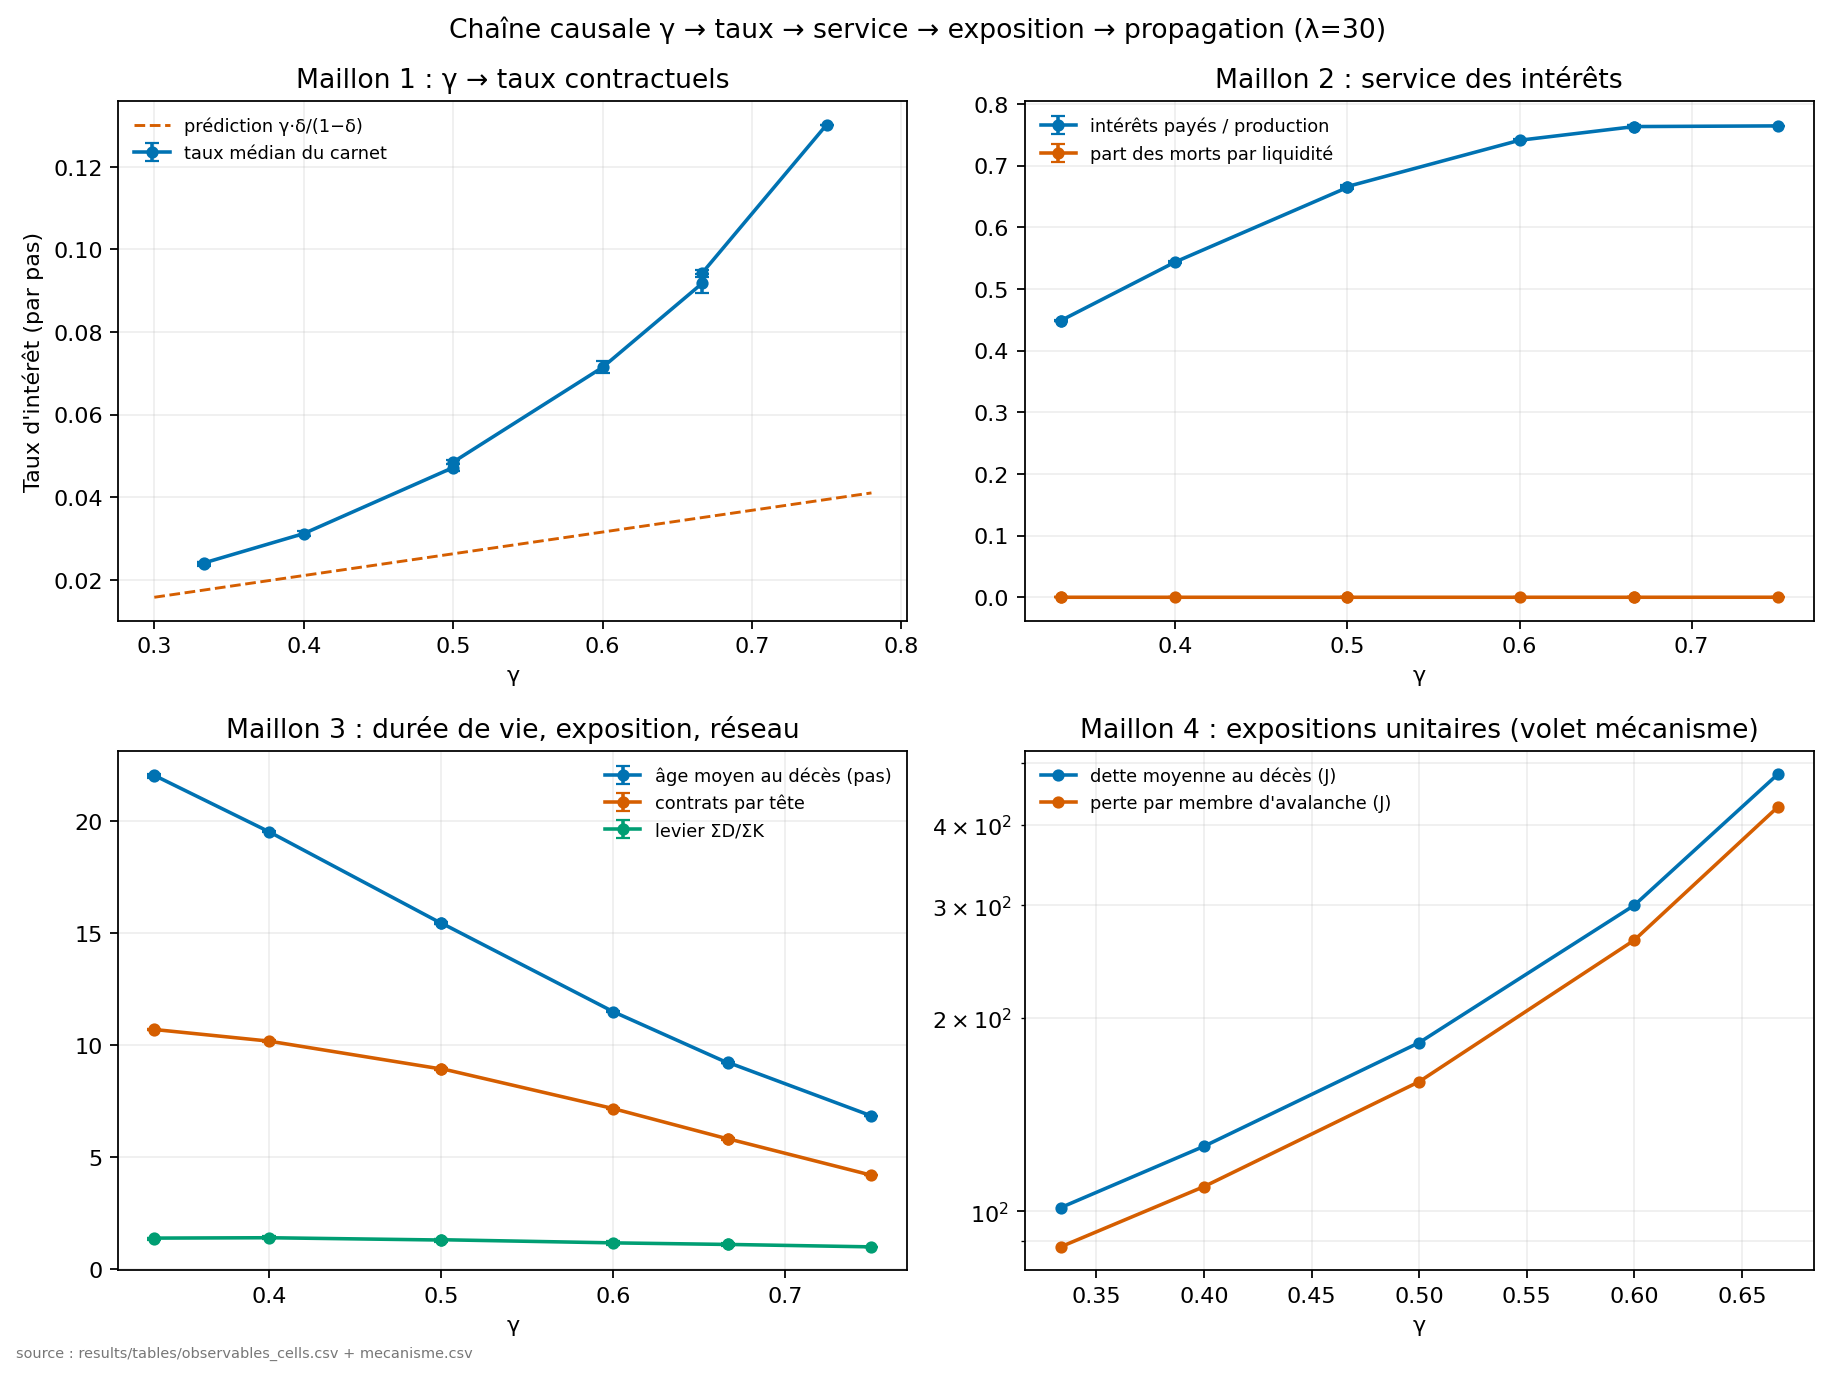
\includegraphics[width=.95\textwidth]{mechanism_chain.png}
\end{center}

La chaîne causale demandée par le cahier des charges est quantifiée
maillon par maillon ($\lambda=30$, exploration, $\gamma$ de $1/3$ à
$2/3$ sauf mention contraire) : $\gamma$ élève le taux médian du carnet,
de $1{,}35$ à $2{,}68$ fois la prédiction autarcique
$\gamma\delta/(1-\delta)$ (croissant avec $\gamma$ ; les contrats se
signent entre entités dont le capital reste en-dessous de $\Kaut$)
$\to$ alourdit le service relatif (intérêts/production : $0{,}45\to
0{,}77$) $\to$ raccourcit les vies (âge moyen au décès : $22{,}0\to6{,}8$
pas, jusqu'à $6{,}8$ pour la sonde $\gamma=0{,}75$, 1 graine) et amincit
le réseau (contrats par tête : $10{,}7\to4{,}2$) $\to$ les expositions
unitaires croissent d'un facteur $\approx5$ (dette moyenne au décès,
perte moyenne par membre d'avalanche : $\approx100\to400$ J, volet
mécanisme, 1 graine par $\gamma$). Ce mécanisme est réel et mesuré ; il
coexiste avec le résultat 2 sans le contredire --- il explique
\emph{comment} $\gamma$ agit sur les flux (et explique au passage
pourquoi le canal de liquidité s'éveille précisément à grand $\gamma$),
tandis que l'ablation établit que son effet net sur $\hat\tau$ transite
majoritairement par l'échelle plutôt que par la forme de la courbe.

\section{Résultats négatifs, limites et garde-fous}

\begin{itemize}
\item \textbf{L'hypothèse de départ (\og la concavité pilote la
pente \fg) est infirmée dans sa forme naïve}, requalifiée en une
conclusion plus profonde et étayée : l'effet observé sur la grille
$\gamma$ à $A=1$ transite très majoritairement par le rapport
adimensionnel $K_0/\Kaut(\gamma,A)$, exactement le type de conclusion
que le cahier des charges anticipait comme possible (\og la pente
dépend d'une combinaison adimensionnelle \fg). Au sens strict des 8
conditions pré-enregistrées, le verdict machine du contraste $\gamma=1/3$
est \textbf{PARTIEL} (échec de la condition n°8, précisément celle qui
révèle la domination d'échelle), pas CONFIRMÉ ; 6 des 8 conditions sont
satisfaites, ce qui distingue nettement ce contraste des deux autres.
\item Les contrastes $\gamma=0{,}6$ et $2/3$ ne satisfont qu'une
minorité des conditions pré-enregistrées ; seul le contraste
$\gamma=1/3$ vs $1/2$ atteint ce niveau de robustesse.
\item Erratum méthodologique découvert en confirmation : la condition
de confirmation n°5 (famille statistique défendable), telle
qu'opérationnalisée, comparait par erreur la loi de puissance
\emph{pure} (déjà rejetée par LRT, $p<4\cdot10^{-33}$, dans les 20 runs
confirmatoires) au log-normal, au lieu de la loi \emph{tronquée}
(modèle primaire). Ce test échoue donc identiquement en cellule et en
centre --- non différentiel, donc non probant contre un contraste
spécifique. Un test de Vuong correctement normalisé, tronquée contre
log-normale (implémenté après l'audit), donne $z=+16$ à $+19$ dans tous
les runs confirmatoires : la famille primaire est massivement
défendable. Le code de décision n'a pas été modifié rétroactivement ;
l'échec littéral et le correctif sont tous deux rapportés.
\item Le test de l'hypothèse structurelle $K_0/\Kaut$ (Résultat 3)
n'établit que la partie nécessaire (théorème d'invariance) ; sa partie
empirique (résidu propre de $\gamma$ à rapport fixé) reste indéterminée
à la précision disponible (3 graines, IC95 $\approx\pm0{,}1$).
\item À $\lambda=100$, la coupure $\hat s_c$ sort systématiquement de
la fenêtre identifiable (hérité de M4B), et $\hat\tau$ y est en réalité
l'exposant de la loi pure ; les scalings de coupure en $\lambda$
reposent sur seulement deux tailles exploitables.
\item Aucune cellule censurée, éteinte ou instable. Le canal de
liquidité, quasi silencieux mais pas rigoureusement nul (17 événements,
uniquement à $\gamma\ge2/3$), reste trop rare pour être caractérisé
quantitativement dans cette campagne ; la question \og que se passe-t-il
si le défaut de service devient dominant \fg{} reste hors du périmètre
exploré (comme dans M4B, où il ne s'activait pleinement qu'à
$\sigma\approx0{,}85$).
\end{itemize}

\section{Réponse à la question ouverte de la mission}

\begin{enumerate}
\item \emph{$\hat\tau$ dépend-il de $\gamma$ dans la réduction
minimale ?} Oui, mesurablement et avec un contraste principal
($\gamma=1/3$ vs $1/2$) satisfaisant 6 des 8 conditions pré-enregistrées.
\item \emph{Cela survit-il aux graines, fenêtres, horizons, tailles ?}
Oui pour ce contraste principal (IC apparié sur graines disjointes,
persistance à $\lambda=100$, stabilité aux fenêtres et à l'horizon
doublé). Non pour $\gamma\ge0{,}6$ (contrastes petits, non robustes en
confirmation).
\item \emph{Concavité, échelle, intérêts, démographie ou réseau ?}
\textbf{Échelle}, dominante : établie par un théorème d'invariance exacte
et par un contrôle d'échelle apparié dont le signe s'inverse de façon
reproductible sur graines d'exploration \emph{et} confirmatoires
disjointes --- via les intérêts et la démographie, qui sont eux-mêmes
pilotés par le rapport $K_0/\Kaut$ plutôt que par $\gamma$ directement.
La part résiduelle propre à la courbure seule, elle, n'est pas tranchée
par cette campagne (Résultat 3).
\item \emph{Quelle plage de pentes sans quitter le régime
stationnaire ?} $\hat\tau\in[1{,}89;2{,}03]$ à $\lambda=30$ sur la
grille explorée ($\gamma\in[1/3,3/4]$, tout stationnaire) --- mais seule
la borne basse ($\gamma=1/3$, $1{,}89$) provient d'un contraste établi
avec robustesse complète ; la borne haute ($\gamma=0{,}6$, $2{,}03$)
vient d'un contraste non confirmé. Cette plage est essentiellement celle
du rapport $K_0/\Kaut$ correspondant, plutôt qu'un effet propre de
$\gamma$.
\item \emph{Si $\gamma$ seul ne suffit pas, quel mécanisme minimal
rend la pente pilotable ?} \textbf{Piloter directement le rapport
$K_0/\Kaut$} (par exemple en fixant $K_0$ à une fraction choisie de
$\Kaut(\gamma,A)$, ou en faisant varier $A$ à $\gamma$ fixé) est le
levier nécessaire et suffisant identifié par l'invariance d'échelle ---
plus direct et plus interprétable que de piloter $\gamma$ pour un effet
équivalent, puisque c'est en réalité le seul canal par lequel $A$ et
$K_0$ peuvent agir sur $\hat\tau$ à $\gamma$ fixé.
\item \emph{Prédictions analytiques simples ?} $\Kaut(\gamma)=19^{1/(1-\gamma)}$
(exact, testé à $10^{-9}$) ; $m(\Kaut)=\gamma\delta/(1-\delta)$ (linéaire
en $\gamma$, exact) ; $K^*(r)=\sqrt{K_\ell K_b}$ (indépendant de $\gamma$,
démontré) ; l'invariance exacte sous $(K,K_0,A)\mapsto(cK,cK_0,c^{1-\gamma}A)$
(démontrée, §Résultat 2), qui implique que $\hat\tau$ ne peut dépendre de
$A,K_0$ qu'à travers $K_0/\Kaut(\gamma,A)$ --- un théorème structurel,
au-delà d'une simple observation de collapse.
\end{enumerate}

% Annexe générée par scripts/make_annexe.py — ne pas éditer à la main.
\section*{Annexe : traçabilité des simulations}
Chaque run est un run Simulation Lab (dossier \code{simulation\_lab\_data/runs/<run\_id>}) ; la correspondance cellule $\to$ runs est dans \code{manifests/*.manifest.json}. Les fits par run sont dans \code{results/metrics/<run\_id>.json} et les agrégats dans \code{results/tables/}.
\begin{small}
\begin{longtable}{llllrrrl}
\toprule
run\_id & plan & cellule & graine & $\gamma$ & $\lambda$ & $T$ & statut\\
\midrule
\endhead
\code{20260727\_160954\_29051328} & benchmark & bench\_g067 & 1 & 0.667 & 30 & 4000 & completed\\
\code{20260727\_160954\_d7c9806c} & benchmark & bench\_g033 & 1 & 0.333 & 30 & 4000 & completed\\
\code{20260727\_161533\_9b2ab740} & pilotes & g040 & 1 & 0.400 & 30 & 4000 & completed\\
\code{20260727\_161533\_dfa5f765} & pilotes & g040 & 2 & 0.400 & 30 & 4000 & completed\\
\code{20260727\_161533\_7ccc4ceb} & pilotes & g040 & 3 & 0.400 & 30 & 4000 & completed\\
\code{20260727\_161533\_be4cd8c8} & pilotes & g033 & 1 & 0.333 & 30 & 4000 & completed\\
\code{20260727\_161533\_128eec20} & pilotes & g033 & 2 & 0.333 & 30 & 4000 & completed\\
\code{20260727\_161533\_986a783a} & pilotes & g033 & 3 & 0.333 & 30 & 4000 & completed\\
\code{20260727\_162133\_2a12e894} & pilotes & g060 & 1 & 0.600 & 30 & 4000 & completed\\
\code{20260727\_162133\_bed8a893} & pilotes & g060 & 2 & 0.600 & 30 & 4000 & completed\\
\code{20260727\_162133\_73b818c9} & pilotes & g060 & 3 & 0.600 & 30 & 4000 & completed\\
\code{20260727\_162110\_0f51704c} & pilotes & g050 & 1 & 0.500 & 30 & 4000 & completed\\
\code{20260727\_162110\_7bedce89} & pilotes & g050 & 2 & 0.500 & 30 & 4000 & completed\\
\code{20260727\_162110\_9eee0426} & pilotes & g050 & 3 & 0.500 & 30 & 4000 & completed\\
\code{20260727\_162603\_57b6df9a} & pilotes & g075\_sonde & 1 & 0.750 & 30 & 4000 & completed\\
\code{20260727\_162531\_d36bad55} & pilotes & g067 & 1 & 0.667 & 30 & 4000 & completed\\
\code{20260727\_162531\_04dfd5f8} & pilotes & g067 & 2 & 0.667 & 30 & 4000 & completed\\
\code{20260727\_162531\_09d69b7e} & pilotes & g067 & 3 & 0.667 & 30 & 4000 & completed\\
\code{20260727\_161533\_be4cd8c8} & taille\_finie & g033 & 1 & 0.333 & 30 & 4000 & completed\\
\code{20260727\_161533\_128eec20} & taille\_finie & g033 & 2 & 0.333 & 30 & 4000 & completed\\
\code{20260727\_161533\_986a783a} & taille\_finie & g033 & 3 & 0.333 & 30 & 4000 & completed\\
\code{20260727\_163104\_a1225eb5} & taille\_finie & g033\_lam10 & 1 & 0.333 & 10 & 8000 & completed\\
\code{20260727\_163104\_b0236ff4} & taille\_finie & g033\_lam10 & 2 & 0.333 & 10 & 8000 & completed\\
\code{20260727\_163104\_fedefddd} & taille\_finie & g033\_lam10 & 3 & 0.333 & 10 & 8000 & completed\\
\code{20260727\_163555\_e4f8c832} & taille\_finie & g040\_lam10 & 1 & 0.400 & 10 & 8000 & completed\\
\code{20260727\_163555\_98e76c0a} & taille\_finie & g040\_lam10 & 2 & 0.400 & 10 & 8000 & completed\\
\code{20260727\_163555\_c70f3ee7} & taille\_finie & g040\_lam10 & 3 & 0.400 & 10 & 8000 & completed\\
\code{20260727\_161533\_9b2ab740} & taille\_finie & g040 & 1 & 0.400 & 30 & 4000 & completed\\
\code{20260727\_161533\_dfa5f765} & taille\_finie & g040 & 2 & 0.400 & 30 & 4000 & completed\\
\code{20260727\_161533\_7ccc4ceb} & taille\_finie & g040 & 3 & 0.400 & 30 & 4000 & completed\\
\code{20260727\_163104\_bef132ad} & taille\_finie & g033\_lam100 & 1 & 0.333 & 100 & 4000 & completed\\
\code{20260727\_163104\_4b9ce8fe} & taille\_finie & g033\_lam100 & 2 & 0.333 & 100 & 4000 & completed\\
\code{20260727\_163104\_68bd7116} & taille\_finie & g033\_lam100 & 3 & 0.333 & 100 & 4000 & completed\\
\code{20260727\_165050\_35fb9cc5} & taille\_finie & g050\_lam10 & 1 & 0.500 & 10 & 8000 & completed\\
\code{20260727\_165050\_00887418} & taille\_finie & g050\_lam10 & 2 & 0.500 & 10 & 8000 & completed\\
\code{20260727\_165050\_c34d4c25} & taille\_finie & g050\_lam10 & 3 & 0.500 & 10 & 8000 & completed\\
\code{20260727\_162110\_0f51704c} & taille\_finie & g050 & 1 & 0.500 & 30 & 4000 & completed\\
\code{20260727\_162110\_7bedce89} & taille\_finie & g050 & 2 & 0.500 & 30 & 4000 & completed\\
\code{20260727\_162110\_9eee0426} & taille\_finie & g050 & 3 & 0.500 & 30 & 4000 & completed\\
\code{20260727\_164035\_9df38b9c} & taille\_finie & g040\_lam100 & 1 & 0.400 & 100 & 4000 & completed\\
\code{20260727\_164035\_c77fba58} & taille\_finie & g040\_lam100 & 2 & 0.400 & 100 & 4000 & completed\\
\code{20260727\_164035\_f8cfdf9a} & taille\_finie & g040\_lam100 & 3 & 0.400 & 100 & 4000 & completed\\
\code{20260727\_165854\_e9868cc7} & taille\_finie & g060\_lam10 & 1 & 0.600 & 10 & 8000 & completed\\
\code{20260727\_165854\_1ed8e88b} & taille\_finie & g060\_lam10 & 2 & 0.600 & 10 & 8000 & completed\\
\code{20260727\_165854\_ad44077d} & taille\_finie & g060\_lam10 & 3 & 0.600 & 10 & 8000 & completed\\
\code{20260727\_162133\_2a12e894} & taille\_finie & g060 & 1 & 0.600 & 30 & 4000 & completed\\
\code{20260727\_162133\_bed8a893} & taille\_finie & g060 & 2 & 0.600 & 30 & 4000 & completed\\
\code{20260727\_162133\_73b818c9} & taille\_finie & g060 & 3 & 0.600 & 30 & 4000 & completed\\
\code{20260727\_165510\_efa1748f} & taille\_finie & g050\_lam100 & 1 & 0.500 & 100 & 4000 & completed\\
\code{20260727\_165510\_1a2ac6e9} & taille\_finie & g050\_lam100 & 2 & 0.500 & 100 & 4000 & completed\\
\code{20260727\_165510\_7cfb5d17} & taille\_finie & g050\_lam100 & 3 & 0.500 & 100 & 4000 & completed\\
\code{20260727\_171108\_35986207} & taille\_finie & g067\_lam10 & 1 & 0.667 & 10 & 8000 & completed\\
\code{20260727\_171108\_1ccc839e} & taille\_finie & g067\_lam10 & 2 & 0.667 & 10 & 8000 & completed\\
\code{20260727\_171108\_708b7b8f} & taille\_finie & g067\_lam10 & 3 & 0.667 & 10 & 8000 & completed\\
\code{20260727\_162531\_d36bad55} & taille\_finie & g067 & 1 & 0.667 & 30 & 4000 & completed\\
\code{20260727\_162531\_04dfd5f8} & taille\_finie & g067 & 2 & 0.667 & 30 & 4000 & completed\\
\code{20260727\_162531\_09d69b7e} & taille\_finie & g067 & 3 & 0.667 & 30 & 4000 & completed\\
\code{20260727\_170313\_45bf4b8f} & taille\_finie & g060\_lam100 & 1 & 0.600 & 100 & 4000 & completed\\
\code{20260727\_170313\_a4a2f4fa} & taille\_finie & g060\_lam100 & 2 & 0.600 & 100 & 4000 & completed\\
\code{20260727\_170313\_f3ec93f2} & taille\_finie & g060\_lam100 & 3 & 0.600 & 100 & 4000 & completed\\
\code{20260727\_171520\_cab04bf8} & taille\_finie & g067\_lam100 & 1 & 0.667 & 100 & 4000 & completed\\
\code{20260727\_171520\_3e7f3be9} & taille\_finie & g067\_lam100 & 2 & 0.667 & 100 & 4000 & completed\\
\code{20260727\_171520\_790e6788} & taille\_finie & g067\_lam100 & 3 & 0.667 & 100 & 4000 & completed\\
\code{20260727\_172713\_c3eaf564} & horizon\_double & g050\_T8000 & 1 & 0.500 & 30 & 8000 & completed\\
\code{20260727\_172713\_8822ea62} & horizon\_double & g050\_T8000 & 2 & 0.500 & 30 & 8000 & completed\\
\code{20260727\_172713\_eca29fdc} & horizon\_double & g050\_T8000 & 3 & 0.500 & 30 & 8000 & completed\\
\code{20260727\_172713\_f6b48923} & horizon\_double & g033\_T8000 & 1 & 0.333 & 30 & 8000 & completed\\
\code{20260727\_172713\_2e2f81ed} & horizon\_double & g033\_T8000 & 2 & 0.333 & 30 & 8000 & completed\\
\code{20260727\_172713\_eb823f56} & horizon\_double & g033\_T8000 & 3 & 0.333 & 30 & 8000 & completed\\
\code{20260727\_174005\_b2c277c8} & horizon\_double & g067\_T8000 & 1 & 0.667 & 30 & 8000 & completed\\
\code{20260727\_174005\_4a0fab1a} & horizon\_double & g067\_T8000 & 2 & 0.667 & 30 & 8000 & completed\\
\code{20260727\_174005\_a7d2ba66} & horizon\_double & g067\_T8000 & 3 & 0.667 & 30 & 8000 & completed\\
\code{20260727\_175504\_85dee157} & confirm & g033\_confirm & 11 & 0.333 & 30 & 4000 & completed\\
\code{20260727\_175504\_da86412e} & confirm & g033\_confirm & 12 & 0.333 & 30 & 4000 & completed\\
\code{20260727\_175504\_5bc07338} & confirm & g033\_confirm & 13 & 0.333 & 30 & 4000 & completed\\
\code{20260727\_175504\_a6f95655} & confirm & g033\_confirm & 14 & 0.333 & 30 & 4000 & completed\\
\code{20260727\_175504\_05396f59} & confirm & g033\_confirm & 15 & 0.333 & 30 & 4000 & completed\\
\code{20260727\_180556\_fc9cc56c} & confirm & g050\_confirm & 11 & 0.500 & 30 & 4000 & completed\\
\code{20260727\_180556\_3b538fea} & confirm & g050\_confirm & 12 & 0.500 & 30 & 4000 & completed\\
\code{20260727\_180556\_ffc1e03b} & confirm & g050\_confirm & 13 & 0.500 & 30 & 4000 & completed\\
\code{20260727\_180556\_bed0e50b} & confirm & g050\_confirm & 14 & 0.500 & 30 & 4000 & completed\\
\code{20260727\_180556\_d0c58064} & confirm & g050\_confirm & 15 & 0.500 & 30 & 4000 & completed\\
\code{20260727\_181536\_0fb74787} & confirm & g060\_confirm & 11 & 0.600 & 30 & 4000 & completed\\
\code{20260727\_181536\_0f37e2cb} & confirm & g060\_confirm & 12 & 0.600 & 30 & 4000 & completed\\
\code{20260727\_181536\_14a294b8} & confirm & g060\_confirm & 13 & 0.600 & 30 & 4000 & completed\\
\code{20260727\_181536\_aa4e0c09} & confirm & g060\_confirm & 14 & 0.600 & 30 & 4000 & completed\\
\code{20260727\_181536\_d787f683} & confirm & g060\_confirm & 15 & 0.600 & 30 & 4000 & completed\\
\code{20260727\_182401\_5542d4b4} & confirm & g067\_confirm & 11 & 0.667 & 30 & 4000 & completed\\
\code{20260727\_182402\_8574a621} & confirm & g067\_confirm & 12 & 0.667 & 30 & 4000 & completed\\
\code{20260727\_182402\_dcc5afba} & confirm & g067\_confirm & 13 & 0.667 & 30 & 4000 & completed\\
\code{20260727\_182402\_1c5fe2b8} & confirm & g067\_confirm & 14 & 0.667 & 30 & 4000 & completed\\
\code{20260727\_182402\_2b851ed1} & confirm & g067\_confirm & 15 & 0.667 & 30 & 4000 & completed\\
\code{20260727\_183204\_0c234778} & ablation\_A & g060\_Anorm & 1 & 0.600 & 30 & 4000 & completed\\
\code{20260727\_183204\_7fea484e} & ablation\_A & g060\_Anorm & 2 & 0.600 & 30 & 4000 & completed\\
\code{20260727\_183204\_0bc048a2} & ablation\_A & g060\_Anorm & 3 & 0.600 & 30 & 4000 & completed\\
\code{20260727\_183204\_b7c8fd58} & ablation\_A & g033\_Anorm & 1 & 0.333 & 30 & 4000 & completed\\
\code{20260727\_183204\_bbb241d1} & ablation\_A & g033\_Anorm & 2 & 0.333 & 30 & 4000 & completed\\
\code{20260727\_183204\_13506a8c} & ablation\_A & g033\_Anorm & 3 & 0.333 & 30 & 4000 & completed\\
\code{20260727\_183808\_16957da0} & ablation\_A & g067\_Anorm & 1 & 0.667 & 30 & 4000 & completed\\
\code{20260727\_183808\_f4780243} & ablation\_A & g067\_Anorm & 2 & 0.667 & 30 & 4000 & completed\\
\code{20260727\_183808\_5ebeae50} & ablation\_A & g067\_Anorm & 3 & 0.667 & 30 & 4000 & completed\\
\code{20260729\_143545\_56cf0dee} & ablation\_A\_confirm & g033\_Anorm\_confirm & 11 & 0.333 & 30 & 4000 & completed\\
\code{20260729\_143546\_0f543b0a} & ablation\_A\_confirm & g033\_Anorm\_confirm & 12 & 0.333 & 30 & 4000 & completed\\
\code{20260729\_143546\_08c4a4d0} & ablation\_A\_confirm & g033\_Anorm\_confirm & 13 & 0.333 & 30 & 4000 & completed\\
\code{20260729\_143546\_0bf46b26} & ablation\_A\_confirm & g033\_Anorm\_confirm & 14 & 0.333 & 30 & 4000 & completed\\
\code{20260729\_143546\_ccb0ded4} & ablation\_A\_confirm & g033\_Anorm\_confirm & 15 & 0.333 & 30 & 4000 & completed\\
\code{20260727\_184355\_b8b2e9f7} & mecanisme & g067\_meca & 1 & 0.667 & 30 & 4000 & completed\\
\code{20260727\_184355\_a1bca015} & mecanisme & g060\_meca & 1 & 0.600 & 30 & 4000 & completed\\
\code{20260727\_184355\_1e0896c8} & mecanisme & g050\_meca & 1 & 0.500 & 30 & 4000 & completed\\
\code{20260727\_184355\_6a568c58} & mecanisme & g040\_meca & 1 & 0.400 & 30 & 4000 & completed\\
\code{20260727\_184355\_e31165e7} & mecanisme & g033\_meca & 1 & 0.333 & 30 & 4000 & completed\\
\code{20260727\_185754\_f69d6fd3} & hypothese\_K0 & k0\_match\_g067 & 1 & 0.500 & 30 & 4000 & completed\\
\code{20260727\_185754\_873a545d} & hypothese\_K0 & k0\_match\_g067 & 2 & 0.500 & 30 & 4000 & completed\\
\code{20260727\_185754\_c39807ce} & hypothese\_K0 & k0\_match\_g067 & 3 & 0.500 & 30 & 4000 & completed\\
\code{20260727\_185754\_bb75a633} & hypothese\_K0 & k0\_match\_g033 & 1 & 0.500 & 30 & 4000 & completed\\
\code{20260727\_185754\_849aa693} & hypothese\_K0 & k0\_match\_g033 & 2 & 0.500 & 30 & 4000 & completed\\
\code{20260727\_185754\_f48f5035} & hypothese\_K0 & k0\_match\_g033 & 3 & 0.500 & 30 & 4000 & completed\\
\bottomrule
\end{longtable}
\end{small}
\noindent Total : 117 exécutions de cellule (102 runs Simulation Lab distincts ; 15 partagés entre plans par identifiant de cellule). Condensat(s) moteur : 932e58643e522d7b (version \code{m4\_2-1}). Rôles des plans : \emph{benchmark} = calibrage de coût (volet 0) ; \emph{pilotes} = exploration grille $\gamma$ (volet 1) ; \emph{taille\_finie} = taille finie $\lambda$ (volet 2) ; \emph{horizon\_double} = robustesse horizon (volet 3) ; \emph{confirm} = confirmation graines 11-15 (volet 4) ; \emph{ablation\_A} = contrôle d'échelle $A_{\mathrm{norm}}$ (volet 5, exploration) ; \emph{ablation\_A\_confirm} = contrôle d'échelle $A_{\mathrm{norm}}$, graines 11-15 (volet 5 étendu) ; \emph{mecanisme} = chaîne causale (volet 6) ; \emph{hypothese\_K0} = hypothèse structurelle $K_0/K^*_{\mathrm{aut}}$ (test ciblé).

\end{document}
